\section{Policy generalization: kind vs.\ phrasing}
\label{sec:generalisation}

Robustness to unseen \emph{tools} (\texttt{heldout\_family}) is not
robustness to unseen \emph{policy kinds} or \emph{phrasings}, and the latter
is the more product-relevant test: a deployment needs the classifier to
apply a customer's own wording, not just handle a new tool under a
training-set policy. ADR 0010 adds two splits: \texttt{heldout\_policy\_kind}
withholds entire predicate kinds (e.g.\ \texttt{forbid\_recipient\_domain})
from training; \texttt{heldout\_policy\_phrasing} withholds one paraphrase
index of every kind the model \emph{did} train on. \texttt{v4} additionally
fixes a renderer defect that left \texttt{privilege\_escalation}
undecidable from text (\S\ref{sec:limitations}).

\begin{table}[tbp]
\centering
\small
\caption{Decoder 2B, macro AUPRC and \texttt{policy\_conflict} AUPRC across
splits, on the v3 (ADR 0010, 15 policy kinds, 2 withheld) and v4 (same data,
\texttt{privilege\_escalation} render fix) generators. v5 (ADR 0011, 30
kinds, 4 withheld) tests whether more kinds let the model generalize the
\emph{shape} of policy-conflict reasoning rather than memorize kinds.
Source: \texttt{docs/results/synthetic-v2/README.md}.}
\label{tab:policy-generalisation}
\begin{tabular}{lcccc}
\toprule
Split & v3 macro & v3 \texttt{policy\_conflict} & v4 macro & v4 \texttt{policy\_conflict} \\
\midrule
test & 0.908 & 0.994 & 0.960 & 0.994 \\
heldout\_family & 0.914 & 0.941 & 0.960 & 0.964 \\
heldout\_policy\_kind & 0.889 & \textbf{0.653} & 0.944 & \textbf{0.752} \\
heldout\_policy\_phrasing & 0.921 & 0.987 & 0.968 & 0.993 \\
\midrule
v5 (30 kinds, 4 withheld) & \multicolumn{4}{c}{\todo{pending: train-2b-b200-v5-recipe.yaml}} \\
\bottomrule
\end{tabular}
\end{table}

\begin{figure}[tbp]
\centering
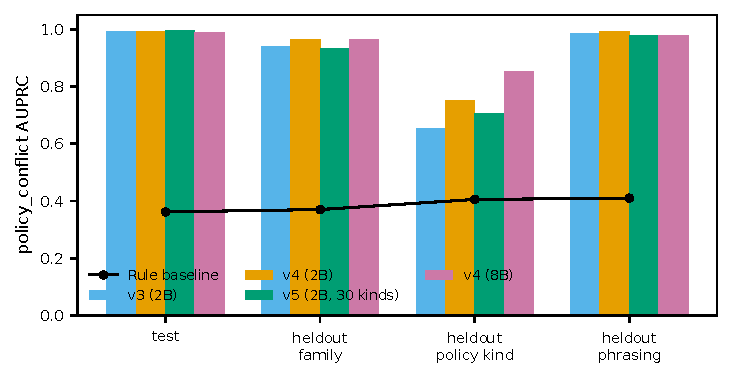
\includegraphics[width=5.5in]{figures/fig_policy_generalisation.pdf}
\caption{Decoder 2B, \texttt{policy\_conflict} AUPRC across splits for the v3
and v4 generators (synthetic data; $n$ per split matches
Table~\ref{tab:policy-generalisation}), with the rule baseline's
\texttt{policy\_conflict} AUPRC on each split shown as a line. The v5 slot is
left blank pending that run. Source:
\texttt{docs/results/synthetic-v2/decoder-2b-v3/}, \texttt{decoder-2b-v4/}.}
\label{fig:policy-generalisation}
\end{figure}

Figure~\ref{fig:policy-generalisation} makes the kind-vs-phrasing asymmetry
visible: bars for test, \texttt{heldout\_family}, and
\texttt{heldout\_policy\_phrasing} sit close together near the ceiling, while
\texttt{heldout\_policy\_kind} drops toward, though still above, the rule
baseline line.

Two very different results. \textbf{Unseen phrasing generalizes.} A
paraphrase index never seen in training leaves \texttt{policy\_conflict} at
0.987--0.993 AUPRC, matching the in-distribution test split (0.994): the
model reads the clause's meaning, not a template id. \textbf{Unseen policy
kinds do not.} With two of fifteen kinds withheld, \texttt{policy\_conflict}
drops to 0.653 (v3) / 0.752 (v4) at a 0.32--0.41 rule-baseline floor -- above
chance but far below every kind seen in training, including under novel
wording. Every other dimension on this split is unaffected, so the model has
learned the fifteen kinds it saw, not the general operation of checking a
predicate against a rendered fact.

The v4 fix also confirms \texttt{privilege\_escalation}'s earlier
AUROC-high/AUPRC-low signature (\S\ref{sec:limitations}) was a data defect,
not a model limit: rendering the deciding
\texttt{authority\_before}/\texttt{authority\_after} values lifts it from
0.505 to 1.000 AUPRC on \texttt{heldout\_family}.

ADR 0011 tests whether more kinds fix kind-generalization: it triples the
inventory to 30 and withholds only 4 (a smaller fraction than v3/v4's
2-of-15). A rise toward the phrasing-generalization level ($\sim$0.99) would
make ``kind'' a learnable unit of generalization; staying in the 0.65--0.75
band despite more diversity would point to a structural limit needing
retrieval-plus-entailment rather than more kinds. Pending at submission time
(Table~\ref{tab:policy-generalisation}, last row).

\FloatBarrier
